\documentclass[]{indojc}

\usepackage{times,amsmath}
\usepackage{amssymb}
\usepackage{graphicx}
\usepackage{lipsum}
\usepackage{url}
\usepackage{color}
\usepackage{fixltx2e}
\usepackage{cite}
\usepackage[T1]{fontenc}
\usepackage[font=small,labelfont=bf]{caption}
\renewcommand{\refname}{Daftar Pustaka}
\usepackage[bahasa]{babel}
%\usepackage{tikz}
% correct bad hyphenation here
\hyphenation{op-tical net-works semi-conduc-tor}
\usepackage{epstopdf}

\begin{document}

% paper title
% Titles are generally capitalized except for words such as a, an, and, as,
% at, but, by, for, in, nor, of, on, or, the, to and up, which are usually
% not capitalized unless they are the first or last word of the title.
% Linebreaks \\ can be used within to get better formatting as desired.
% Do not put math or special symbols in the title.

\makeatletter
\title{IoT on Heart Arrhyhtmia Real Time Monitoring}

%Please change "Sample Paper with indojc Class for Indonesian Journal on Computing" with your title bellow:
\newcommand{\Title}{\reverseit{IoT on Heart Arrhyhtmia Real Time Monitoring}}

\author{%
{Muhammad Alif Akbar{\small $~^{\#1}$}, \and Satria Mandala{\small $~^{*2}$}}%
\vspace{1.6mm}\\
\fontsize{10}{10}\selectfont\itshape
$^{\#}$\,department of Informatics Engineering, School of Computing, Telkom University\\
Bandung, Jawa Barat, Indonesia\\
\fontsize{9}{9}\selectfont\upshape
$^{1}$\, maakbar@student.telkomuniversity.ac.id\\
$^{2}$\, satriamandala@telkomuniversity.ac.id%
}

%Please change "First Author" below into you paper's first author
\newcommand\Author{Muhammad Alif Akbar}


\maketitle
\thispagestyle{firststyle}

% As a general rule, do not put math, special symbols or citations
% in the abstract or keywords.
\def\abstractname{Abstract}
\def\keywordsname{Keywords}
\begin{abstract}
An abstract of no more than 200 words should state the purposes of the study, procedures, findings and conclusions. It should be written in Times New Roman with font size of 9. Abstract should be followed by four to eight key words to assist cross-indexing. The key words should be ordered alphabetically and separated by commas. For your paper to be published in the journal, you must use this document as both an instruction set and as a template into which you can type your own text.  If your paper does not conform to the required format, you will be asked to fix it. In the paper, authors are suggested to present their articles in the sections structure: Introduction - Previous Study/Literature Review - The Proposed Method/Algorithm/Procedure specifically designed (optional) - Research Method - Results and Discussion - Conclusion. Authors may present complex proofs of theorems or non-obvious proofs of correctness of algorithms after introduction section (obvious theorems and straightforward proofs of existing theorems are not needed).
\end{abstract}

\begin{keywords}
Indo-JC, journal, \LaTeX, template.
\end{keywords}
$~$\\
\def\abstractname{Abstrak}
\def\keywordsname{Kata Kunci}
\begin{abstract}
Abstrak berisikan tidak lebih dari 200 kata yang meliputi tujuan dari penelitian, prosedur, temuan dan kesimpulan. Ukuran dan jenis huruf untuk abstak adalah Times New Roman dengan ukuran 9. Bagian abstrak ditutup dengan 4-9 kata kunci abstrak. Kata kunci ini berfungsi untuk membantu pengindexan. Kata kunci harus diurutkan secara alphabet dan dipisahkan dengan koma. Agar makalah Anda dapat dipublish di journal kami, Anda harus menggunakan dokumen ini baik sebagai himpunan petunjuk maupun sebagai template. Jika makalah Anda tidak sesuai dengan format yang diberikan, maka paper Anda akan dikembalikan agar dapat diperbaiki. Dalam makalah ini, penulis disarankan untuk menyajikan artikel dengan struktur sebagai berikut: Pendahuluan - Kajian Pustaka  - Metode Usulan/ Algoritma/ Prosedur yang didesain secara spesifik (pilihan) - Metodologi Penelitian - Hasil dan Pembahasan - Kesimpulan. Penulis dapat menyajikan bukti teorema yang kompleks atau bukti yang non-obvious dari algoritma setelah bagian pendahuluan (teorema yang sudah jelas mauun bukti langsung tidak perlu dicantumkan kembali).
\end{abstract}

\begin{keywords}
Indo-JC, jurnal, \LaTeX, template.
\end{keywords}


\section{Introduction}
\TSoCPARstart{T}{his} demo file is a template for Indonesian Journal on Computing (Indo-JC) produced under \LaTeX\ using indojc.cls. The template describes page style used in Indo-JC and sections that should be written in the manuscript. Authors who want to submit their manuscript to Indo-JC must follow this template. This is important to maintain the quality of the journal. Therefore, if one paper does not conform to the required template, the author will be asked to fix it.

\subsection{Content of Introduction Section}
In introduction, the context of the study and state the precise objective should be explained. An Introduction should contain the following three parts: background, the problem, and proposed solution. In explaining the background, authors have to make clear what the context is. Ideally, authors should give an idea of the state-of-the art of the field the report is about. The problem also need to described clearly so that readers able to understand why they should proceed reading. Authors also need to describe the proposed solution so that readers able to point out what are the novel aspects of authors work. Authors should place the paper in proper context by citing relevant papers. 

\subsection{Page Layout and Style}
The manuscript must use a page size corresponding to A4. The margins must be set 3 cm for each top, bottom, left and right margins. The manuscript also must be in one column format. All paragraphs must be indented. All paragraphs must be justified, i.e. both left-justified and right- justified.

Times New Roman or Times font should be used for the manuscript. Font size 10 is used in general, except for title (24), author information (11), abstract (9), and caption for figures and tables (8). More details on the font style used can be seen in Table \ref{tab:font-sizes}.

\begin{table}[!h]
\centering

    \caption{Font Sizes for Manuscripts}   
    \label{tab:font-sizes}
    \begin{small}
    \begin{tabular}{|c|l|l|l|}
    \hline
    {\bfseries Font} & \multicolumn{3} {c|} {\bfseries Appearance (in Times New Roman or Times} \\
    \cline{2-4}
    {\bfseries Size} & {\bfseries  Regular}         & {\bfseries Bold}     & {\bfseries Italic}           \\
    \hline
    8         & table caption (in	&		& reference item	\\
              & Small Caps),		&		& (partial)		\\
              &	figure caption,		&		&			\\
              &	reference item		&		&			\\
    \hline
    9         & author email address,	& abstract body & abstract heading	\\
              &	cell in a table 		&		&    (also in Bold)	\\
    \hline
    10        & level-1 heading  (in 	&		& level-2 heading,      \\
              & Small Caps),		&		& level-3 heading,	\\
              &	paragraph		&		& author affiliation	\\
    \hline
    11        &	author name		&		&			\\
    \hline
    24        & title			&		&			\\
    \hline
    \end{tabular}
    \end{small} 
\end{table}

All title and author details must be in single-column format and must be centered. Every word in a title must be capitalized except for short minor
words such as ``a'', ``an'', ``and'', ``as'', ``at'', ``by'', ``for'', ``from'',
``if'', ``in'', ``into'', ``on'', ``or'', ``of'', ``the'', ``to'', ``with''.  To avoid confusion, the family name must be written as the last part of each author name (e.g. Mary J. Smith). Each affiliation must include, at the very least, the name of the company and the name of the country where the author is based (e.g. Telkom University, Indonesia).  

For section headings, no more than 3 levels of headings should be used. All headings must be in 10pt font. Every word in a heading must be capitalized except for short minor words as listed above.

\subsubsection{Level-1 Heading}
A level-1 heading must be in Small Caps, centered and numbered using uppercase Roman numerals. Please be noted that "Acknowledgment" and "References" are level-1 headings which must not be numbered.

\subsubsection{Level-2 Heading}
A level-2 heading must be in Italic, left-justified and numbered using an uppercase alphabetic letter followed by a period. 

\subsubsection{Level-3 Heading} 
A level-3 heading must be indented, in Italic and numbered with an Arabic numeral followed by a right parenthesis. The level-3 heading must end with a colon. The body of the level-3 section immediately follows the level-3 heading in the same paragraph. For example, this paragraph begins with a level-3 heading.

\subsection{Equations, Figures, and Tables}
Number equations consecutively with equation numbers in parentheses flush with the right margin, as in (\ref{eq:satu}). Be sure that the symbols in your equation have been defined before the equation appears or immediately following. 

\begin{equation}
S(N,K) = \frac{\sum_{i=1}^n(w_i\times sim(f_N,f_K))}{\sum_{i=1}^nw_i}
\label{eq:satu}
\end{equation}


Figures and tables must be centered in the column. Please check all figures in your paper both on screen and on a black-and-white hard copy. When you check your paper on a black-and-white hard copy, please ensure that: the colors used in each figure contrast well, the image used in each figure is clear, and all text labels in each figure are legible. Figures must be numbered using Arabic numerals. Figure captions must be in 8 pt regular font. Captions of a single line must be centered whereas multi-line captions must be justified. Captions with figure numbers must be placed after their associated figures. Example of a figure can be seen in Fig. \ref{fig:oneexample}.

\begin{figure}[!t]
\centering
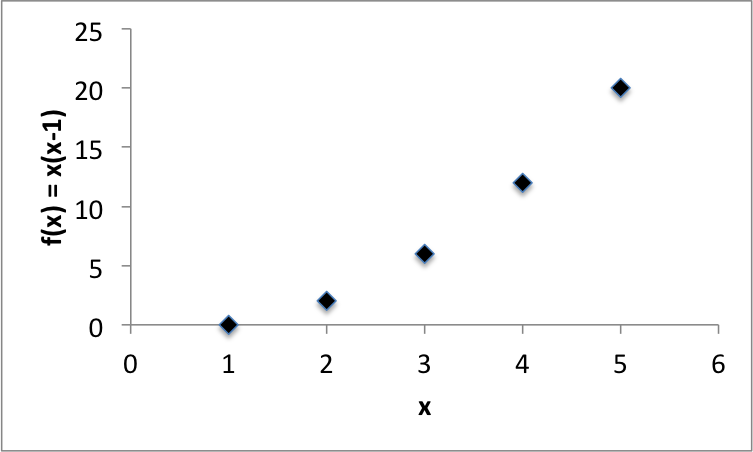
\includegraphics[width=2.5in, keepaspectratio=true]{fig_example.png}
\caption{Example of a figure.}
\label{fig:oneexample}
\end{figure}

Tables must be numbered using uppercase Roman numerals. Table captions must be centered and in 8 pt regular font with Small Caps. Every word in a table caption must be capitalized except for short minor words as listed before. Captions with table numbers must be placed before their associated tables, as shown in \ref{tab:font-sizes}.

\subsection{References}
References are written using plain style as seen in the reference section in this example file. Only for example, citation in the manuscript should be written like this \cite{kopka1999guide} or for many citations can be written as \cite{lamport1994latex,swope1982computer,huo2007short}. In this file, references is organized using bibtex. You can see the bibtex file in myreference.bib including some bibtex style examples can be used.


\section{Literature Review}
The aim of a literature review is to show the readers that authors have read, and have a good grasp of, the main published work concerning a particular topic or question in the field. It is very important to note that the review should not be simply a description of what others have published in the form of a set of summaries, but should take the form of a critical discussion, showing insight and an awareness of differing arguments, theories and approaches. It should be a synthesis and analysis of the relevant published work, linked at all times to your own purpose and rationale.

\section{Research Method}
The presentation of the experimental methods should be clear and complete in every detail facilitating reproducibility by other scientists.

\section{Results and Discussion}
The presentation of results should be simple and straightforward. This section reports the most important findings, including results of statistical analysis as appropriate and comparisons to other research results. Results given in figures should not be repeated in tables. This is where Authors should explain in words what he/she/they discovered in the research. It should be clearly laid out and in a logical sequence. This section should be supported suitable references.

\section{Conclusion}
Summarize sentences the primary outcomes of the study in a paragraph. Explain if the claims in this section supported by the results, and if they seem reasonable. Also, describe whether the result support or contradict previous theories, and explain how the research has moved the body of scientific knowledge forward. 

% use section* for acknowledgment
\section*{Acknowledgment}
The authors would like to thank...

%Use following code if you use bibtex

\bibliographystyle{plain}
\bibliography{References}{}


% Without bibtex
%\begin{thebibliography}{1}
%
%\bibitem{one}
%H.~Kopka and P.~W. Daly, \emph{A Guide to \LaTeX}, 3rd~ed.\hskip 1em plus
%  0.5em minus 0.4em\relax Harlow, England: Addison-Wesley, 1999.
%\bibitem{books1}
%J. K. Author, "Title of chapter in the book," in \emph{Title of His Published Book}, xth ed. City of Publisher, Country if not
%\bibitem{books2}
%USA: Abbrev. of Publisher, year, ch. x, sec. x, pp. xxx-xxx.
%\bibitem{onlinejournal}
%Author. (year, month). Title. \emph{Journal. volume (issue)}, pages. Available: site/path/file 
%\bibitem{proceeding}
%J. K. Author, "Title of paper," in \emph{Abbreviated Name of Conf.}, City of Conf., Abbrev. State (if given), year, pp. xxxxxx.
%\bibitem{dissertation}
%J. K. Author, "Title of dissertation," Ph.D. dissertation, Abbrev. Dept., Abbrev. Univ., City of Univ., Abbrev. State, year.
%
%\end{thebibliography}


\end{document}


